\documentclass[11pt,a4paper]{article}
\usepackage[margin=2.5cm]{geometry}
\usepackage{graphicx}
\usepackage{amsmath}
\usepackage{booktabs}
\usepackage{caption}
\usepackage{subcaption}
\usepackage[colorlinks=true,linkcolor=blue,citecolor=blue,urlcolor=blue]{hyperref}

\captionsetup{font=small,labelfont=bf}
\graphicspath{{figures/}}

\title{Natural Convection in a Square Cavity:\\
Nek5000 Benchmark at $\mathrm{Ra}=10^{3}$ and $\mathrm{Ra}=10^{6}$\\
\large Archive \texttt{nek5000-ncsq}, cases \texttt{Ra1e3} and \texttt{Ra1e6}}
\author{Hai Lu Lin}
\date{August 17, 2026}

\begin{document}
\maketitle

\begin{abstract}
Steady natural convection of air ($\mathrm{Pr}=0.71$) in a differentially heated
square cavity is computed with the spectral-element code Nek5000 at Rayleigh
numbers $\mathrm{Ra}=10^{3}$ (case \texttt{Ra1e3}) and $\mathrm{Ra}=10^{6}$
(case \texttt{Ra1e6}), and validated against the spectral-element discontinuous
Galerkin lattice Boltzmann (SEDG--LBM) results of Patel et al.~\cite{patel2014}
and the benchmark solutions collected therein. At $\mathrm{Ra}=10^{3}$ the
mid-plane temperature profiles are indistinguishable from the reference data and
the mean and extremal Nusselt numbers agree with the converged SEDG--LBM values
to within $0.01\%$, and with the older de~Vahl~Davis benchmark to within
$0.11\%$. At
$\mathrm{Ra}=10^{6}$ the mean Nusselt number is $0.40$--$0.63\%$ above the
reference values. This offset is traced to the two-significant-figure rounding
of the prescribed transport properties in the \texttt{Ra1e6} parameter file,
which raises the effective Rayleigh number by $2.0\%$ and accounts for
essentially all of the observed difference.
\end{abstract}

\section{Introduction}
Natural convection in a differentially heated square cavity is a standard
benchmark for buoyancy-driven incompressible flow solvers. This report documents
two Nek5000 cases, \texttt{Ra1e3} and \texttt{Ra1e6}, which reproduce the cavity
flow at $\mathrm{Ra}=10^{3}$ and $\mathrm{Ra}=10^{6}$ respectively, both at
$\mathrm{Pr}=0.71$. Results are compared with the SEDG--LBM computation of Patel
et al.~\cite{patel2014} and with the reference solutions that paper validates
against: the multiple-relaxation-time lattice Boltzmann results of Wang et
al.~\cite{wang2013}, the finite-difference benchmark of de~Vahl
Davis~\cite{davis1983}, the lattice Boltzmann results of Dixit and
Babu~\cite{dixit2006}, and the high-accuracy pseudo-spectral solutions of
Le~Qu\'er\'e~\cite{lequere1991}.

The two cases share a mesh, a \texttt{SIZE} file and a user-routine file; they
differ only in the transport properties set in \texttt{ncsq.par}. Together they
bracket the transition from a conduction-dominated regime at $\mathrm{Ra}=10^{3}$
to a convection-dominated, boundary-layer regime at $\mathrm{Ra}=10^{6}$. The
two cases were named \texttt{ncsq4} and \texttt{ncsq5} in the original numbered
run series and are referred to by those names in earlier draft write-ups; they
were renamed on archiving to identify them by Rayleigh number.

\section{Problem description}
The domain is the unit square $[0,1]^{2}$. All four walls are no-slip,
$\mathbf{u}=\mathbf{0}$. The left wall is held at the hot temperature
$T_h=1$ and the right wall at the cold temperature $T_c=0$; the horizontal
walls are adiabatic, $\partial T/\partial y=0$. The fluid starts at rest with
$T\equiv0$. Under the Boussinesq approximation the governing equations are
\begin{align}
\nabla\cdot\mathbf{u} &= 0,\\
\rho\left(\frac{\partial\mathbf{u}}{\partial t}
  + \mathbf{u}\cdot\nabla\mathbf{u}\right)
  &= -\nabla p + \mu\nabla^{2}\mathbf{u} + \rho g \beta (T-T_0)\,\hat{\mathbf{e}}_y,\\
\rho c_p\left(\frac{\partial T}{\partial t}
  + \mathbf{u}\cdot\nabla T\right) &= k\,\nabla^{2}T .
\end{align}
The governing parameters are
\begin{equation}
\mathrm{Ra} = \frac{g\beta\,(T_h-T_c)\,L^{3}}{\nu\alpha},
\qquad
\mathrm{Pr} = \frac{\nu}{\alpha} = \frac{\mu c_p}{k},
\label{eq:RaPr}
\end{equation}
where $\nu=\mu/\rho$ is the kinematic viscosity and $\alpha = k/(\rho c_p)$ the
thermal diffusivity. The reference quantities are set to unity,
$\rho = c_p = \beta = L = 1$ and $\Delta T = T_h - T_c = 1$, with $g=9.81$.
Inverting~\eqref{eq:RaPr} gives the properties that must be prescribed for a
target $(\mathrm{Ra},\mathrm{Pr})$ pair:
\begin{equation}
\mu = \sqrt{\frac{g\,\mathrm{Pr}}{\mathrm{Ra}}},
\qquad
k = \sqrt{\frac{g}{\mathrm{Pr}\,\mathrm{Ra}}} .
\label{eq:props}
\end{equation}
The buoyancy term is applied in \texttt{userf} as the acceleration
$f_y = g\,T$, which Nek5000 multiplies by the density. Because
$T_0=(T_h+T_c)/2$ is constant, omitting it from the forcing contributes only a
uniform hydrostatic acceleration that is absorbed into the pressure gradient
and does not affect the velocity field.

Table~\ref{tab:params} lists the properties prescribed in the two parameter
files. The values are those actually present in \texttt{ncsq.par}, rounded to
the precision at which they were entered; Section~\ref{sec:rounding} examines
the consequences of that rounding.

\begin{table}[htbp]
\centering
\caption{Prescribed non-dimensional properties for the two cases. All other
reference quantities are unity, with $g=9.81$.}
\label{tab:params}
\begin{tabular}{lccc}
\toprule
Case & Target $\mathrm{Ra}$ & $\mu$ & $k$\\
\midrule
\texttt{Ra1e3} & $10^{3}$ & $8.35\times10^{-2}$ & $1.175\times10^{-1}$\\
\texttt{Ra1e6} & $10^{6}$ & $2.6\times10^{-3}$ & $3.7\times10^{-3}$\\
\bottomrule
\end{tabular}
\end{table}

\section{Numerical setup}
Both cases use Nek5000~\cite{fischer2008} (version 20.0-dev), a spectral-element
method solver,
with the stress formulation of the viscous terms. The mesh is generated by
\texttt{genbox} from \texttt{ncsq.box} and consists of $10\times10=100$ uniform
quadrilateral elements at polynomial order $N=7$ (\texttt{lx1}~$=8$
Gauss--Lobatto--Legendre points per direction per element), giving $6\,400$ grid
points. The time step is adapted to a target CFL number of $0.4$ and the
velocity residual tolerance is $10^{-6}$. Both runs are advanced to $t=100$
convective time units, at which point the fields are steady; \texttt{Ra1e3}
reached this in $20\,018$ steps and \texttt{Ra1e6} in $38\,927$ steps. All
results below are taken from the final state.

Note that this resolution is considerably coarser than that of the reference
computation, which used $E=256$ elements at $N=5$ for $\mathrm{Ra}\le10^{5}$ and
$E=576$ at $N=9$ for $\mathrm{Ra}=10^{6}$~\cite{patel2014}. The implications are
discussed in Section~\ref{sec:rounding}.

The Nusselt number on the hot wall is defined following Ref.~\cite{patel2014} as
\begin{equation}
\mathrm{Nu}_0 = \int_0^1 q_x\big|_{x=0}\,\mathrm{d}y,
\qquad
q_x = u_x T - \frac{\partial T}{\partial x},
\label{eq:nu}
\end{equation}
which reduces to $\mathrm{Nu}_0 = -\int_0^1 (\partial T/\partial x)|_{x=0}\,
\mathrm{d}y$ at the no-slip wall. Here $\mathrm{Nu}_0^{\max}$ and
$\mathrm{Nu}_0^{\min}$ denote the local extrema of the integrand along that
wall. These quantities were evaluated in post-processing from the final field
file.

\section{Results at \texorpdfstring{$\mathrm{Ra}=10^{3}$}{Ra=1e3}}

\subsection{Flow and temperature fields}
Figure~\ref{fig:ra3fields} shows the computed streamlines and isotherms. The
flow forms a single clockwise recirculation cell, driven by fluid rising at the
hot wall and sinking at the cold wall. The isotherms remain close to vertical,
indicating that heat transfer is still conduction-dominated at this Rayleigh
number, with only a mild convective distortion. Both fields agree qualitatively
with Fig.~3(a) of Ref.~\cite{patel2014}.

\begin{figure}[htbp]
\centering
\begin{subfigure}[b]{0.49\textwidth}
  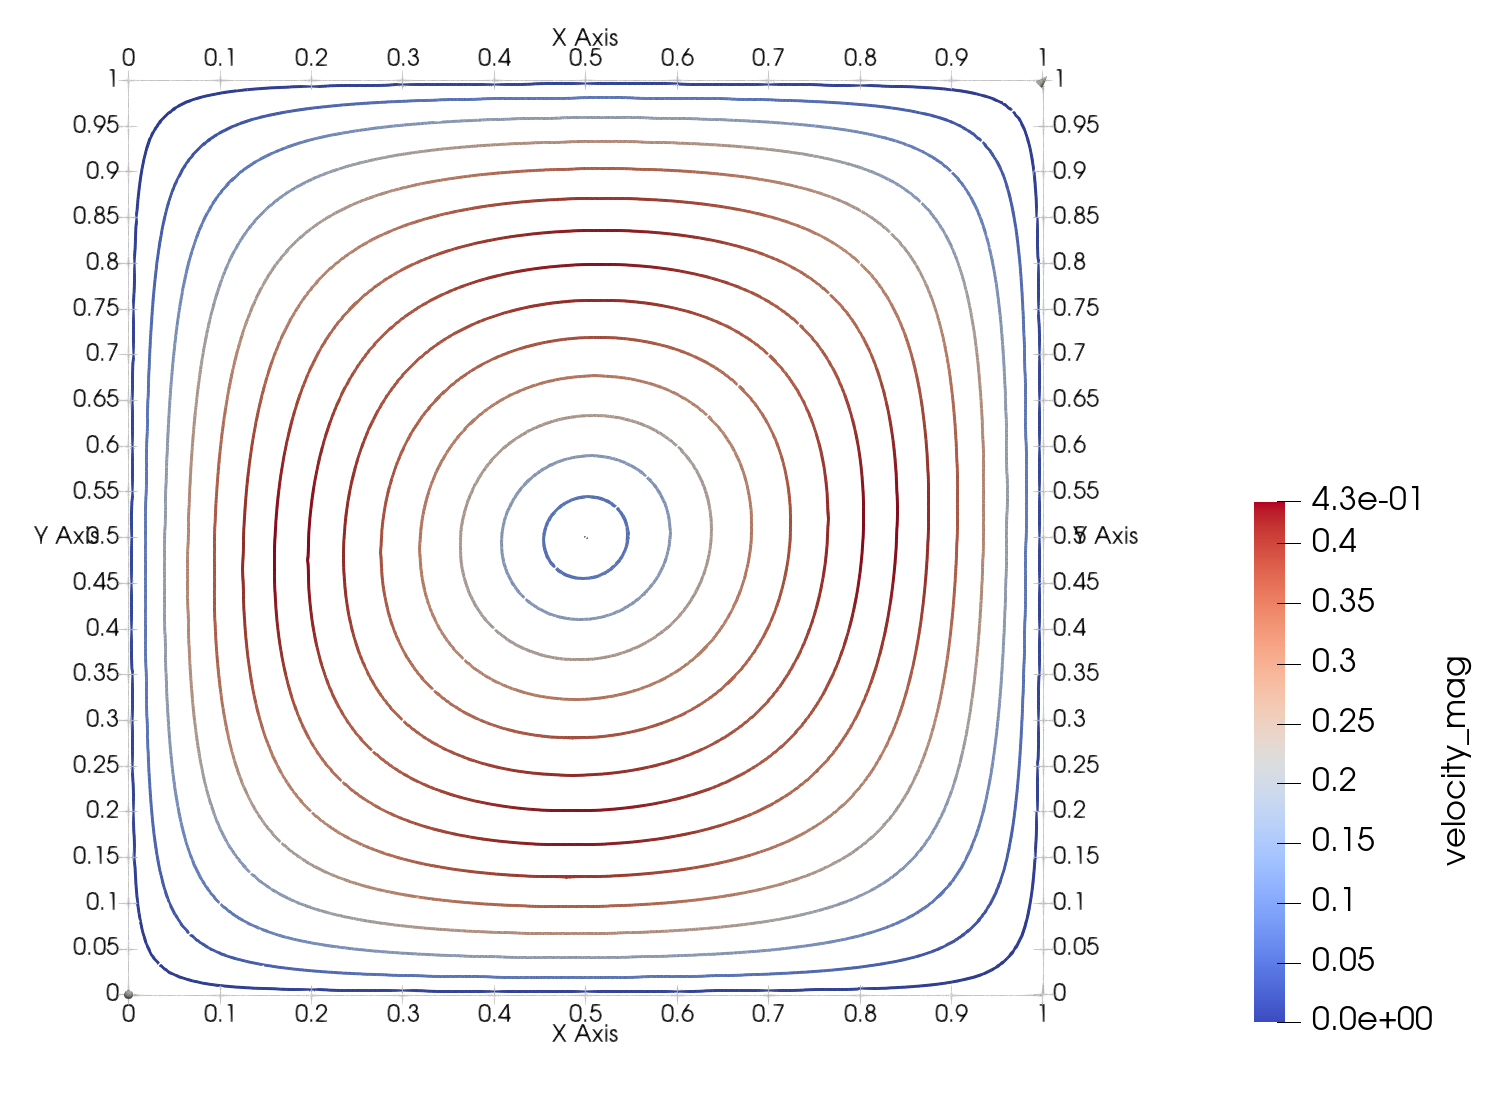
\includegraphics[width=\textwidth]{ra3_streamlines.png}
  \caption{Streamlines, colored by velocity magnitude.}
\end{subfigure}
\hfill
\begin{subfigure}[b]{0.49\textwidth}
  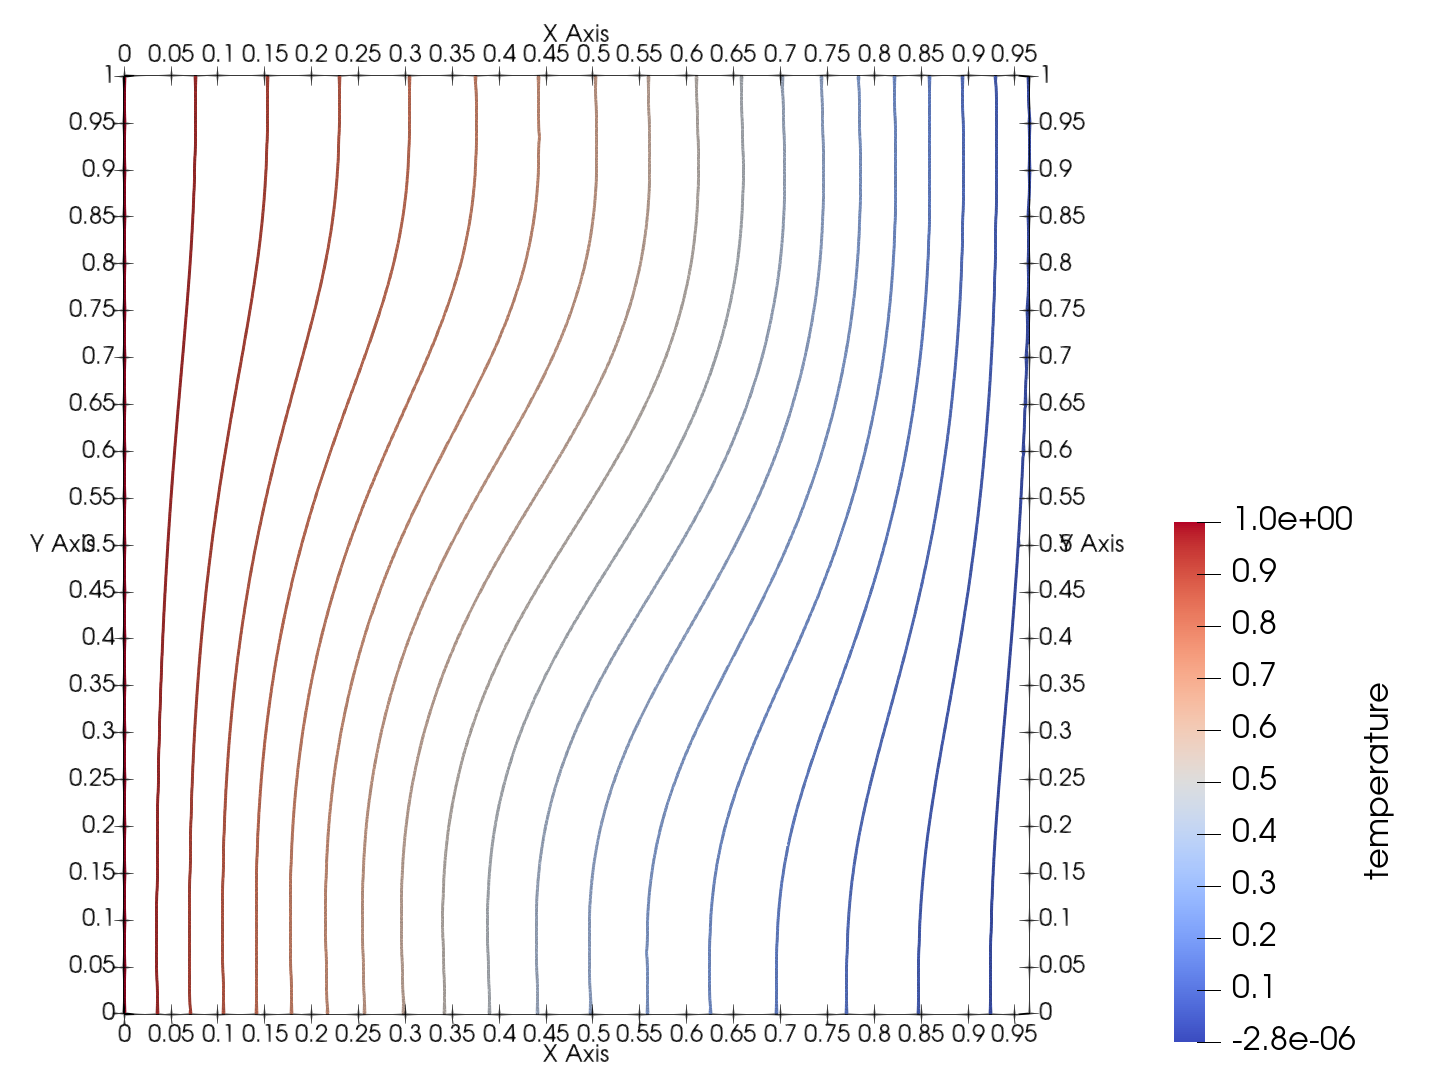
\includegraphics[width=\textwidth]{ra3_isotherms.png}
  \caption{Isotherms, $T\in[0,1]$.}
\end{subfigure}
\caption{Steady-state flow (left) and temperature (right) fields at
$\mathrm{Ra}=10^{3}$, $\mathrm{Pr}=0.71$ (case \texttt{Ra1e3}).}
\label{fig:ra3fields}
\end{figure}

\subsection{Mid-plane temperature profiles}
Figure~\ref{fig:profiles} compares the temperature profiles along the vertical
mid-plane ($x=0.5$) and the horizontal mid-plane ($y=0.5$) with data digitized
from Fig.~4 of Ref.~\cite{patel2014}. The Nek5000 profiles pass through the
reference points along both lines. The horizontal mid-plane profile is nearly
linear, again consistent with the conduction-dominated regime.

\begin{figure}[htbp]
\centering
\begin{subfigure}[b]{0.49\textwidth}
  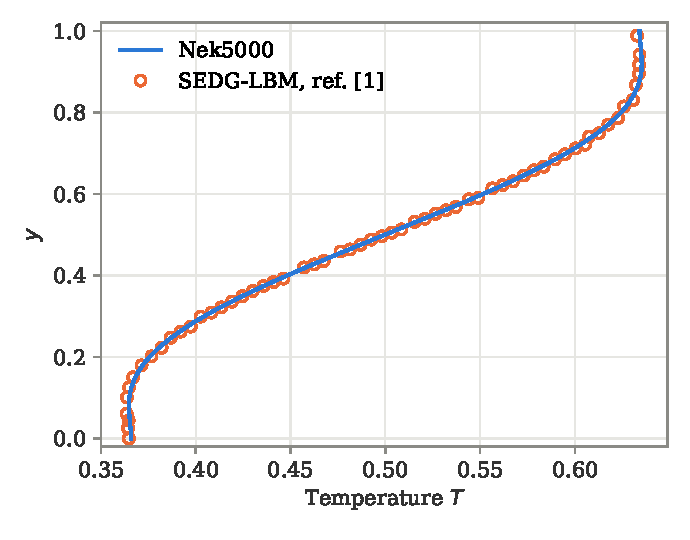
\includegraphics[width=\textwidth]{ra3_profile_x05.pdf}
  \caption{Vertical mid-plane, $x=0.5$.}
\end{subfigure}
\hfill
\begin{subfigure}[b]{0.49\textwidth}
  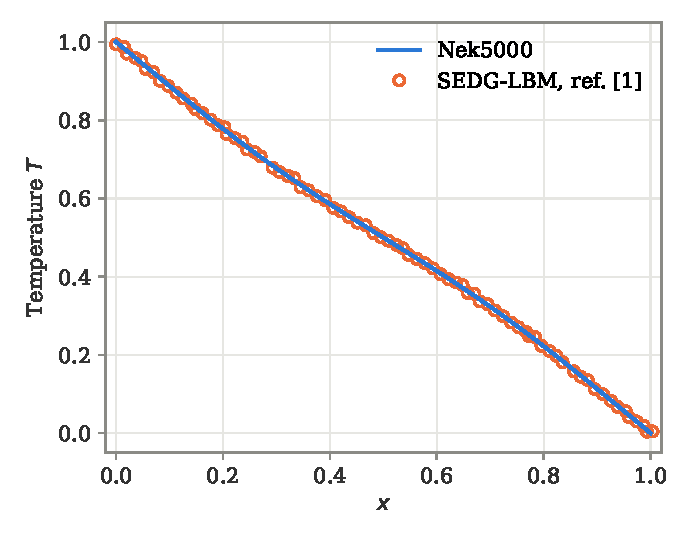
\includegraphics[width=\textwidth]{ra3_profile_y05.pdf}
  \caption{Horizontal mid-plane, $y=0.5$.}
\end{subfigure}
\caption{Temperature profiles along the cavity mid-planes at
$\mathrm{Ra}=10^{3}$: Nek5000 (solid line) versus SEDG--LBM reference
data~\cite{patel2014} (open circles).}
\label{fig:profiles}
\end{figure}

\subsection{Nusselt number}
Table~\ref{tab:nu3} compares the mean Nusselt number on the hot wall and its
local extrema against the SEDG--LBM result at $N=9$~\cite{patel2014}, the
lattice Boltzmann result of Wang et al.~\cite{wang2013}, and the benchmark
solution of de~Vahl~Davis~\cite{davis1983}. The Nek5000 mean value matches the
converged SEDG--LBM and Wang et al.\ results to four significant digits
($-0.004\%$); all three quantities lie within $0.01\%$ of those two references.
The deviation from the older de~Vahl~Davis benchmark is larger but still small,
at most $0.11\%$ (on $\mathrm{Nu}_0^{\min}$), reflecting the lower precision of
that 1983 finite-difference solution rather than a difference in the present
result.

\begin{table}[htbp]
\centering
\caption{Mean, maximum, and minimum Nusselt numbers on the hot wall at
$\mathrm{Ra}=10^{3}$, $\mathrm{Pr}=0.71$.}
\label{tab:nu3}
\begin{tabular}{lccc}
\toprule
 & $\overline{\mathrm{Nu}}_0$ & $\mathrm{Nu}_0^{\max}$ & $\mathrm{Nu}_0^{\min}$\\
\midrule
SEDG--LBM ($N=9$)~\cite{patel2014} & 1.1178 & 1.5063 & 0.6913\\
Wang et al.~\cite{wang2013} & 1.1178 & 1.5063 & 0.6912\\
de Vahl Davis~\cite{davis1983} & 1.117 & 1.505 & 0.692\\
\textbf{Nek5000 (present)} & \textbf{1.11776} & \textbf{1.50622} & \textbf{0.691258}\\
\bottomrule
\end{tabular}
\end{table}

\section{Results at \texorpdfstring{$\mathrm{Ra}=10^{6}$}{Ra=1e6}}

\subsection{Flow and temperature fields}
Figure~\ref{fig:ra6fields} shows the streamlines and isotherms at
$\mathrm{Ra}=10^{6}$. The flow structure is qualitatively different from the
$\mathrm{Ra}=10^{3}$ case: the single central vortex has broken into a
horizontally elongated core containing two secondary eddies, and the motion is
confined to thin boundary layers along the vertical walls. The isotherms are
nearly horizontal through the core, showing the stable thermal stratification
characteristic of convection-dominated cavity flow, and steepen sharply near
the hot and cold walls. Both features reproduce Fig.~5(a) of
Ref.~\cite{patel2014}.

\begin{figure}[htbp]
\centering
\begin{subfigure}[b]{0.49\textwidth}
  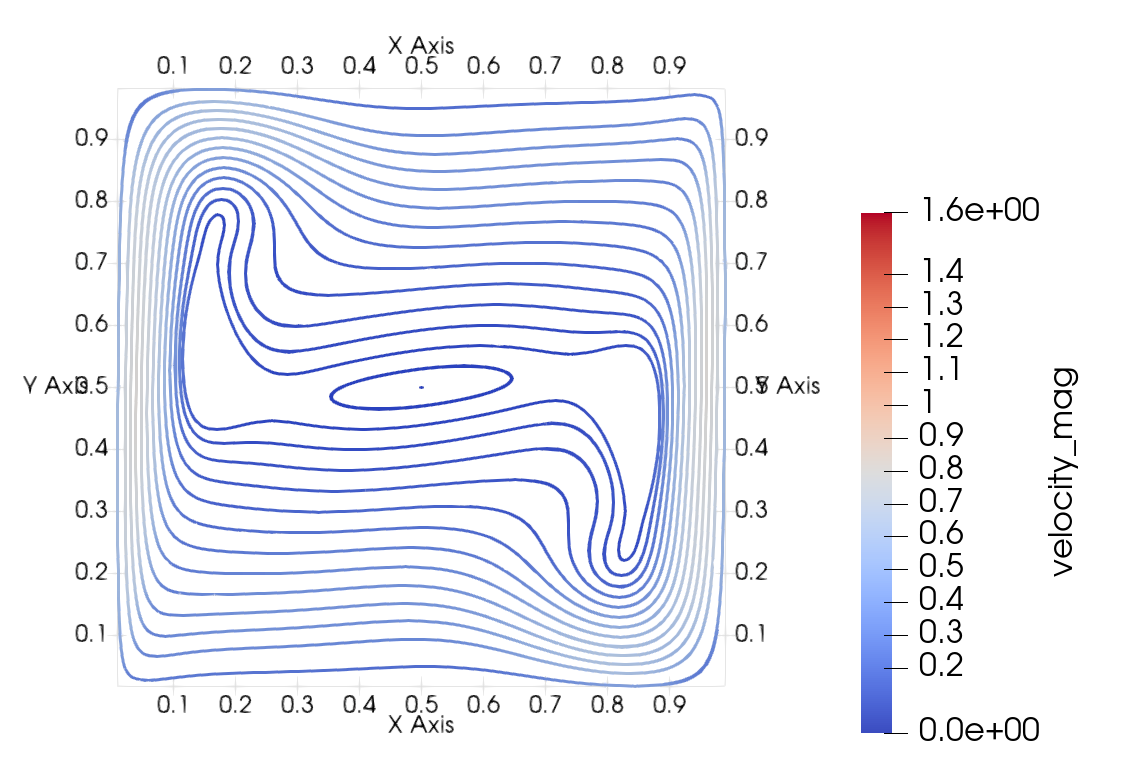
\includegraphics[width=\textwidth]{ra6_streamlines.png}
  \caption{Streamlines, colored by velocity magnitude.}
\end{subfigure}
\hfill
\begin{subfigure}[b]{0.49\textwidth}
  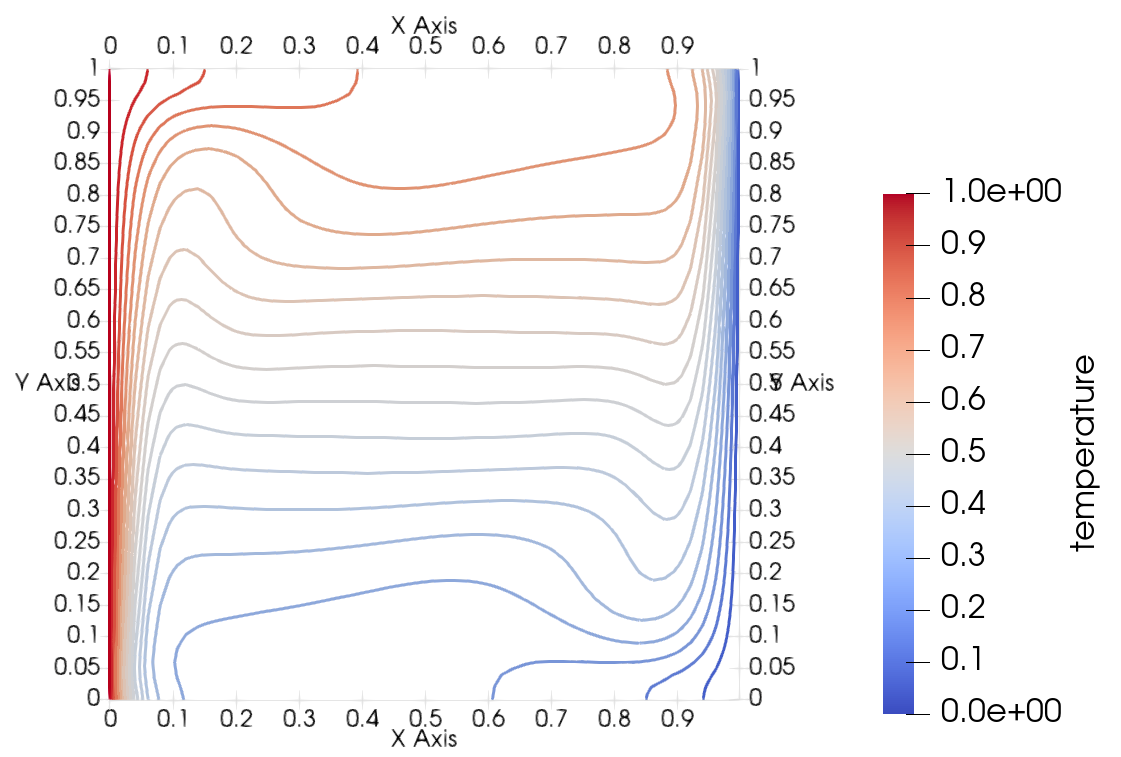
\includegraphics[width=\textwidth]{ra6_isotherms.png}
  \caption{Isotherms, $T\in[0,1]$.}
\end{subfigure}
\caption{Steady-state flow (left) and temperature (right) fields at
$\mathrm{Ra}=10^{6}$, $\mathrm{Pr}=0.71$ (case \texttt{Ra1e6}).}
\label{fig:ra6fields}
\end{figure}

\subsection{Nusselt number}
Table~\ref{tab:nu6} compares the computed mean Nusselt number with the four
reference values tabulated in Ref.~\cite{patel2014}. The Nek5000 value is
$0.40$--$0.63\%$ higher than the references, which themselves span a range of
$0.23\%$. The offset is one to two orders of magnitude larger than at
$\mathrm{Ra}=10^{3}$ and is examined in the next section.

\begin{table}[htbp]
\centering
\caption{Mean Nusselt number on the hot wall at $\mathrm{Ra}=10^{6}$,
$\mathrm{Pr}=0.71$. The last column gives the deviation of the present result
from each reference.}
\label{tab:nu6}
\begin{tabular}{lcc}
\toprule
 & $\overline{\mathrm{Nu}}_0$ & Deviation of present result\\
\midrule
SEDG--LBM~\cite{patel2014} & 8.820 & $+0.46\%$\\
Wang et al.~\cite{wang2013} & 8.8192 & $+0.47\%$\\
Dixit and Babu~\cite{dixit2006} & 8.805 & $+0.63\%$\\
Le Qu\'er\'e~\cite{lequere1991} & 8.8252 & $+0.40\%$\\
\textbf{Nek5000 (present)} & \textbf{8.86074} & ---\\
\bottomrule
\end{tabular}
\end{table}

\section{Effect of rounding the prescribed properties}
\label{sec:rounding}
The transport properties in Table~\ref{tab:params} were entered into
\texttt{ncsq.par} at finite precision, so the Rayleigh and Prandtl numbers the
solver actually integrates differ slightly from the nominal targets. Recovering
them by substituting the prescribed $\mu$ and $k$ back
into~\eqref{eq:RaPr} gives the effective values in Table~\ref{tab:effective}.

\begin{table}[htbp]
\centering
\caption{Effective governing parameters implied by the properties actually
prescribed in each parameter file, compared with the nominal targets.}
\label{tab:effective}
\begin{tabular}{lcccc}
\toprule
Case & Target $\mathrm{Ra}$ & Effective $\mathrm{Ra}$ & Effective $\mathrm{Pr}$
 & $\Delta\mathrm{Ra}$\\
\midrule
\texttt{Ra1e3} & $10^{3}$ & $999.9$ & $0.7106$ & $-0.01\%$\\
\texttt{Ra1e6} & $10^{6}$ & $1.0198\times10^{6}$ & $0.7027$ & $+1.98\%$\\
\bottomrule
\end{tabular}
\end{table}

For \texttt{Ra1e3} the properties were entered to four significant figures and
the effective Rayleigh number is within $0.01\%$ of the target, which is
consistent with the four-digit agreement in Table~\ref{tab:nu3}. For
\texttt{Ra1e6}, however, $\mu$ was rounded to two significant figures:
$2.6\times10^{-3}$ instead of the exact $2.63915\times10^{-3}$ required
by~\eqref{eq:props}, a $1.48\%$ reduction. Together with the $0.46\%$ reduction
in $k$, this raises the effective Rayleigh number by $1.98\%$ and lowers the
effective Prandtl number by $1.03\%$.

The sensitivity of the Nusselt number to this shift can be estimated from the
reference data itself. Fitting a power law $\mathrm{Nu}_0\propto
\mathrm{Ra}^{\,n}$ to the SEDG--LBM values at $\mathrm{Ra}=10^{6}$ and $10^{7}$
in Ref.~\cite{patel2014} gives $n=0.273$. A $+1.98\%$ change in Rayleigh number
then predicts a $+0.53\%$ change in $\overline{\mathrm{Nu}}_0$, which is the
same size as the $+0.40$ to $+0.63\%$ deviations in Table~\ref{tab:nu6}.
Property rounding therefore accounts for essentially the whole discrepancy, and
the \texttt{Ra1e6} result is better read as a correct solution of a slightly
different problem than as an error in the solver or the discretization.

Two caveats apply. First, no grid-refinement study was performed for either
case, so a resolution contribution cannot be excluded. At $\mathrm{Ra}=10^{6}$
the thermal boundary layer thickness is roughly $L/(2\,\mathrm{Nu}_0)\approx
0.056$, which spans about half an element; the Gauss--Lobatto--Legendre
clustering places approximately four points within it, which is adequate but
not generous, and the present mesh is far coarser than the $E=576$, $N=9$
resolution used in Ref.~\cite{patel2014}. Second, the $1.03\%$ shift in Prandtl
number has been neglected in the estimate above, as the Nusselt number depends
only weakly on $\mathrm{Pr}$ for $\mathrm{Pr}=O(1)$.

The practical remedy is to enter the properties at full precision, that is
$\mu = 2.63915\times10^{-3}$ and $k = 3.71711\times10^{-3}$ for
$\mathrm{Ra}=10^{6}$, $\mathrm{Pr}=0.71$, and to repeat the run before drawing
quantitative conclusions at this Rayleigh number.

\section{Conclusions}
The Nek5000 spectral-element setup for natural convection in a differentially
heated square cavity has been validated at two Rayleigh numbers.

At $\mathrm{Ra}=10^{3}$ (case \texttt{Ra1e3}) the agreement is excellent: the
mid-plane temperature profiles are indistinguishable from the SEDG--LBM
reference data of Patel et al.~\cite{patel2014}, and the mean and extremal
hot-wall Nusselt numbers agree with the converged SEDG--LBM and Wang et al.\
values to within $0.01\%$, and with the de~Vahl~Davis benchmark to within
$0.11\%$. This validates the non-dimensional Boussinesq formulation, the
property relations~\eqref{eq:props}, and the buoyancy forcing $f_y = gT$.

At $\mathrm{Ra}=10^{6}$ (case \texttt{Ra1e6}) the flow structure and thermal
stratification are reproduced correctly, and the mean Nusselt number falls
$0.40$--$0.63\%$ above the reference values. This offset is explained by the
two-significant-figure rounding of $\mu$ in the parameter file, which raises the
effective Rayleigh number by $1.98\%$ and, at the reference sensitivity
$\mathrm{Nu}_0\propto\mathrm{Ra}^{0.273}$, predicts a $+0.53\%$ shift in
$\overline{\mathrm{Nu}}_0$. Rerunning \texttt{Ra1e6} with full-precision
properties, and adding a grid-refinement study, would confirm this and is
recommended before the case is used quantitatively.

\begin{thebibliography}{9}

\bibitem{patel2014}
S.~S. Patel, M.~Min, K.~C. Uga, and T.~Lee,
``A spectral-element discontinuous Galerkin lattice Boltzmann method for
simulating natural convection heat transfer in a horizontal concentric
annulus,'' \emph{Computers \& Fluids}, vol.~95, pp.~197--209, May 2014,
doi:\href{https://doi.org/10.1016/j.compfluid.2014.02.021}{10.1016/j.compfluid.2014.02.021}.

\bibitem{wang2013}
J.~Wang, D.~Wang, P.~Lallemand, and L.-S. Luo,
``Lattice Boltzmann simulations of thermal convective flows in two
dimensions,'' \emph{Computers \& Mathematics with Applications}, vol.~65,
no.~2, pp.~262--286, 2013.

\bibitem{davis1983}
G.~de~Vahl~Davis,
``Natural convection of air in a square cavity: A benchmark numerical
solution,'' \emph{International Journal for Numerical Methods in Fluids},
vol.~3, no.~3, pp.~249--264, 1983.

\bibitem{dixit2006}
H.~N. Dixit and V.~Babu,
``Simulation of high Rayleigh number natural convection in a square cavity
using the lattice Boltzmann method,'' \emph{International Journal of Heat and
Mass Transfer}, vol.~49, no.~3, pp.~727--739, 2006.

\bibitem{lequere1991}
P.~Le~Qu\'er\'e,
``Accurate solutions to the square thermally driven cavity at high Rayleigh
number,'' \emph{Computers \& Fluids}, vol.~20, no.~1, pp.~29--41, 1991.

\bibitem{fischer2008}
P.~Fischer, J.~Lottes, D.~Pointer, and A.~Siegel,
``Petascale algorithms for reactor hydrodynamics,'' \emph{Journal of Physics:
Conference Series}, vol.~125, no.~1, 012076, 2008.

\end{thebibliography}

\end{document}
